% Présentation de TeX et LaTeX
\small

\section{Présentation de \TeX\ et \LaTeX}

\subsection{Qu'est-ce que \TeX\ et \LaTeX?}

% Qu'est-ce que TeX?
\begin{frame}{Qu'est-ce que \TeX?}
	\begin{columns}
		\begin{HEClegende}{Donald Knuth}
			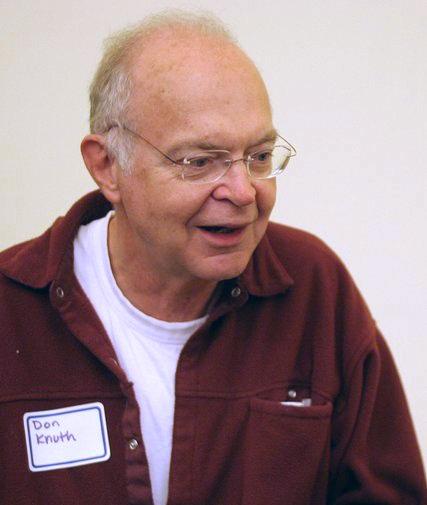
\includegraphics[width=.9\textwidth,keepaspectratio=true]{KnuthAtOpenContentAlliance.jpg}
			
			{\tiny\faCreativeCommons\ Jacob Appelbaum, 2005}
		\end{HEClegende}
		\begin{HECcontenuLegende}
			\begin{itemize}
				\item Un système de mise en page (\emph{typesetting}) et de préparation de documents
				créé par Donald Knuth.
				\item «Le système le plus puissant pour produire des ouvrages scientifiques et
				techniques d'une grande qualité typographique.»\footnote{Kopka \& Daly, p. 6}
				\item Un système mature, stable et complet, considéré comme exempt de bogues.
				\item Un ensemble de commandes très primitives parfaites pour la typographie et
				des fonctions de programmation.
				\item «\emph{typesetter-level program}»
			\end{itemize}
		\end{HECcontenuLegende}
	\end{columns}
\end{frame}

% Qu'est-ce que LaTeX?
\begin{frame}{Qu'est-ce que \LaTeX?}
	\begin{columns}
		\begin{HEClegende}{Leslie Lamport}
			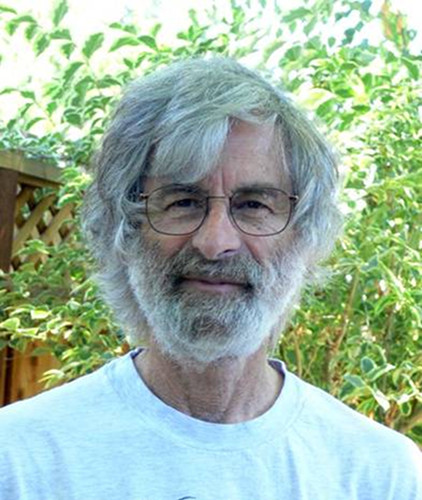
\includegraphics[width=.9\textwidth,keepaspectratio=true]{Leslie_Lamport.jpg}
		\end{HEClegende}
		\begin{HECcontenuLegende}
			\begin{itemize}
				\item Un ensemble de macro-commandes créées par Leslie Lamport pour faciliter l'utilisation de \TeX.
				\item Ne requiert aucune connaissance préalable de la typographie en général et de \TeX\ en particulier.
				\item Langage de balisage (\emph{Markup Language}) typographique et logique pour indiquer la mise en forme du texte (pensez au HTML).
				\item Langage multiplateforme, identique d'un système d'exploitation à l'autre, et extensible par l'ajout de \emph{packages}.
				\item «\emph{author-level program}»
			\end{itemize}
		\end{HECcontenuLegende}
	\end{columns}
\end{frame}

\subsection{Processus de création d'un document \LaTeX}

% Rédiger avec une nouvelle perspective
\begin{frame}[c]{Rédiger avec une nouvelle perspective}
	
	\begin{itemize}
		\item Vous rédigez votre document en texte brut et utilisez des commandes pour décrire
			\textbf{ce que votre texte représente} et \textbf{non pas ce à quoi il doit ressembler}.
		\item Vous vous concentrez sur votre \textbf{contenu}.
		\item Vous laissez \LaTeX\ faire son travail, c'est-à-dire s'occuper du \textbf{contenant}.
	\end{itemize}
	
\end{frame}

% Processus de création d'un document LaTeX
\begin{frame}[c]{Processus de création d'un document \LaTeX}


\end{frame}